\documentclass{article}
\usepackage[utf8]{inputenc}
\usepackage{amsfonts}
\usepackage{amsmath}
\usepackage{amsthm}
\usepackage{color}
\usepackage[dvipsnames]{xcolor}
\usepackage{graphicx}
\usepackage{setspace}
\usepackage{multicol}
\graphicspath{ {./images/} }
\usepackage{listings}
\makeatletter
\renewcommand\@biblabel[1]{}
\makeatother
\lstset{frame=tb,
  language=python,
  aboveskip=5mm,
  belowskip=5mm,
  showstringspaces=false,
  columns=flexible,
  basicstyle={\small\ttfamily},
  numbers=none,
  numberstyle=\tiny\color{blue},
  keywordstyle=\color{red},
  commentstyle=\color{gray},
  stringstyle=\color{ForestGreen},
  breaklines=true,
  breakatwhitespace=true,
  tabsize=3}
                
\title{Principal Component Analysis and Facial Recognition}
\author{Jocelyn Hsieh and Kelly Ding}
\date{December 2022}

\begin{document}
\maketitle
\pagebreak

\begin{center}
    \Huge Cover Letter
\end{center}
We worked on this paper mostly in sections. Jocelyn worked on the derivations and the python example, while Kelly worked on the eigenface application.

Jocelyn: Mainly in the derivation of maximum variance formulation, I got a lot of feedback on providing more definitions for methods that might not have been familiar. For instance, I added the definition of partial derivative, which is used minimally in the section involving Lagrange multipliers. I did my best to include more explanation for these methods that might not have been super familiar. In general, I tried to include more explanation in the formulation sections, since these are very cumulative and involve lots of random small details that can be difficult to recall and/or have an intuition for. 

I also received feedback that the minimum error formulation would be helpful, so I wrote this section to show that this formulation gave the same result as the maximum variance formulation. This ended up being really helpful to show that the eigenvectors that serve as principal components should correspond to the largest eigenvalues, which wasn't initially clear before. I tried to format this similarly to the maximum variance formulation so that the reader would feel more comfortable with it. One difficulty was that this section had a lot of small steps that I wanted to show involving summation and dot products, since this is what took me longest to understand. Hopefully my explanations there are sufficient.

I also received feedback that the programming section was a bit too long, but since I plan to use this document for myself, since I do want to do more with PCA, I kept most of the explanation (the code took a long time to write and understand). I also spent a good chunk of time making the equations more readable, since in the formulation sections, there are a lot of equations that can make the reading very dense. 

Kelly: As for the eigenface section, we mostly got feedback to add more definitions, formatted similarly to the PCA part, and add more depth. So, I tried to break down the process of calculating and utilizing eigenfaces following Turk and Pentland's paper. I also tried to make the whole explanation more mathematical and did my best to tie back the process to what we have already expained in the PCA section. 

We also received feedback that we should cite our sources, which in retrospect we should have started doing earlier (but didn't).


\pagebreak

\section{Introduction}
How can we distinguish faces? As humans, we can easily detect differences in facial features, head shape, and facial structure. Theoretically, we can then break down the detection method and train an algorithm to do the same. However, this process is incredibly complicated. The algorithm must consider countless variables that change with different faces. With so much information, we must find a way to only focus on the important variables. Luckily with Principal Component Analysis, we are given a method to reduce the number of variables to focus on, while still maintaining range of data. 

\section{Principal Component Analysis}
Principal Component Analysis (PCA) is a method for feature extraction, which allows us to find the main features of data. PCA is particularly helpful for reducing dimensionality: suppose we are given data that may change according to many variables, then PCA allows us to reduce this data to only the variables that best explain the data. 

\vspace{2mm}
\noindent We first define a principal component.

\vspace{3mm}

\noindent\fbox{%
    \parbox{\textwidth}{%
        \textbf{Definition.} \textit{Principal Component}. A vector whose span best fits the data. The next best vectors, which are orthogonal to the primary principal component, are also principal components. 
    }%
}

\vspace{3mm}
\noindent Given this definition of a principal component, we now seek a way to find the principal components. That is, which components capture the spread in the data, or the variance? To answer this question, we first introduce a formal definition of variance.

\vspace{3mm}

\noindent\fbox{%
    \parbox{\textwidth}{%
        \textbf{Definition.} \textit{(Sample) Variance}. A measure of spread given some data points, which can be measured by the sum of each point's distance from the mean. Let $N$ be the total number of data points, and $\mu$ be the mean.
        
        Then the variance of this data is: 
        \center{$\sigma^2 = \frac{1}{N}\sum_{n=1}^{N}(x_n - \mu)^2$ \hspace{3mm}(Peck et al., 2008, p.191)}
    }%
}

\vspace{3mm}
\noindent  We seek to show that maximizing the variance of projections onto a lower dimension will yield the principal components. In doing so, we retain the most important features of each point. Then the directions of the lower-dimensional space must give meaningful information on the data, since we have eliminated dimensions that provide no useful information on the data. With this intuition, we are now ready to derive the principal components.


\subsection{Maximum Variance Formulation}
Suppose we have N data points, which we represent as vectors $\mathbf{x_n}$, such that $n \in \{1, 2, \cdots, N\}$ and $\mathbf{x_n} \in \mathbb{R}^D$: the data point is in dimension $D$ and thus determined by $D$ variables. For simplicity, we project these $N$ data points onto a subspace of dimension 1, which we say is spanned by $\mathbf{w}$, with unit length 1.

\vspace{2mm}
\noindent The amount that each vector $\mathbf{x_n}$ projects onto $\mathbf{w}$ is given by $\hat{x} = \frac{\mathbf{w} \cdot \mathbf{x_n}}{\mathbf{w \cdot w}}$. Recall that $\mathbf{w}$ has length 1, so $\mathbf{w} \cdot \mathbf{w} = ||w||^2 = 1$. Then $\hat{x}_n = \mathbf{w \cdot x_n}$. Recall from the definition of dot product that this is equivalently: $\hat{x}_n = \mathbf{w^T}\mathbf{x_n}$.

\vspace{2mm}
\noindent Suppose that $\bar{\mathbf{x}}$ is the mean of the $N$ data points, then its projection is $\hat{\bar{\mathbf{x}}} = \mathbf{w^T}\mathbf{\bar{\mathbf{x}}}$, from similar reasoning to above.

\vspace{2mm}
\noindent Now we can apply the definition of variance, from above. Recall that we will want to maximize this value. 

\vspace{-3mm}
\[
\begin{minipage}{.5\linewidth}
  \centering
  $
  \setstretch{1.5}
  \begin{array}{l@{{}\mathrel{=}{}}l}
    \sigma^2 & \frac{1}{N} \sum_{n = 1}^{N}(\hat{\mathbf{x_n}} - \hat{\bar{\mathbf{x}}})^2 \\[\jot]
    &\frac{1}{N} \sum_{n=1}^{N}(\mathbf{w^{T}x_{n}} - \mathbf{w^{T}\bar{x}})^2 \\[\jot]
     &\frac{1}{N}\sum_{n=1}^{N}(\mathbf{w^{T}x_{n} - w^{T}\bar{x}})(\mathbf{w^{T}x_{n} - w^{T}\bar{x}})
  \end{array}$
\end{minipage}%
\begin{minipage}{.35\linewidth}
  \centering
  $
  \setstretch{1.5}
  \begin{array}{r}
    \\[\jot]
    \text{Substituting in known values.}\\[\jot]
    \text{Expanding.}
  \end{array}$
\end{minipage}
\]


\vspace{2mm}
\noindent Recall that dot product is commutative, so $\mathbf{w^{T}x} = \mathbf{w\cdot x} = \mathbf{x \cdot w} = \mathbf{x^{T}w}$.\newline
Then $\sigma^2 = \frac{1}{N}\sum_{n=1}^{N}(\mathbf{w^{T}x_{n} - w^{T}\bar{x}})(\mathbf{x^{T}_{n}w - \bar{x}^{T}w})$. Factoring out $\mathbf{w, w^T}$:\newline
$=\frac{1}{N}\sum_{n=1}^{N}\mathbf{w^T}(\mathbf{x_n - \bar{x}})(\mathbf{x_{n}^{T} - \bar{x}^T})\mathbf{w}$.

\vspace{2mm}
\noindent In order to continue simplifying this expression for variance, we must introduce a new term. 

\vspace{3mm}

\noindent\fbox{%
    \parbox{\textwidth}{%
        \textbf{Definition.} \textit{Variance-Covariance Matrix (Covariance Matrix)}. Covariance generally measures the variance between two variables: if variable $X$ increases as $Y$ increases, then they have positive covariance, and if $X$ increases as $Y$ decreases, then they have negative covariance. Let $\mu_1, \mu_2$ be the mean for $X, Y$, respectively. Covariance for two variables is given as $\frac{1}{N}\sum_{n=1}^{N}(x_n - \mu_1)(y_n - \mu_2)$ (Blitzstein & Hwang, 2019, p.326).
        
        \vspace{2mm}
        Now suppose that $\mathbf{X}$ is a vector in $\mathbb{R}^D$, where each element in the vector is a variable. Then we measure variance for each $X_i, X_j: i, j \in \{1, 2, \cdots, D\}$, which we represent as a matrix:
        
        \vspace{2mm}
          \begin{center}
              $\begin{bmatrix}
        Cov(X_1, X_1) & Cov(X_2, X_1) & \cdots & Cov(X_D, X_1)\\
        Cov(X_1, X_2) & Cov(X_2, X_2) & \cdots & Cov(X_D, X_2)\\
        \vdots & & \ddots & \vdots \\
        Cov(X_1, X_D) & Cov(X_2, X_D) & \cdots & Cov(X_D, X_D)
        \end{bmatrix}$
          \end{center}
        
        \vspace{2mm}
        Analogous to the definition of covariance of two variables, we define this matrix:\newline
        $\mathbf{S} = \frac{1}{N}\sum_{n=1}^{N}(\mathbf{x_n - \bar{x}})(\mathbf{x_n - \bar{x}})^T$.\hfill (Lay et al., 2016, p. 428)
    }%
}

\vspace{3mm}
\noindent From our definitions, we note two properties of covariance and the covariance matrix.

\vspace{3mm}
\noindent\fbox{%
    \parbox{\textwidth}{%
        \textbf{Property.}
        \noindent \textit{1. Commutativity of Covariance} (Blitzstein & Hwang, 2019, 327). We simply note that since multiplication is commutative,
        \begin{flalign*}
            \text{Cov(X, Y)} &= \frac{1}{N}\sum_{n=1}^{N}(x_n - \mu_1)(y_n - \mu_2) \\&= \frac{1}{N}\sum_{n=1}^{N}(y_n - \mu_2)(x_n - \mu_1) \\&=  \text{Cov(Y, X)}
        \end{flalign*}
        
        \noindent \textit{2. Symmetry of Covariance Matrix}. Note from how the covariance matrix is represented that across the main diagonal, we have values Cov($X_i, X_j$) and Cov($X_j, X_i$). From above, we know these values are the same, thus the covariance matrix is symmetric.
    }%
}

\vspace{3mm}
\noindent Now we can simplify our expression for variance to $\sigma^2 = \mathbf{w^{T}Sw}$. To find the maximum of this, we use the method of Lagrange Multipliers.


\vspace{3mm}
\noindent\fbox{%
    \parbox{\textwidth}{%
        \textbf{Definition.} \textit{Partial Derivative}. The partial derivative of a function $f(x, y)$ with respect to $x$ is the ordinary derivative of $f$, keeping $y$ constant.

        \begin{center}
            $f_{x}(x, y) = \lim\limits_{h\to 0}\frac{f(x+h, y)-f(x, y}{h}$
        \end{center}
        
        We will need to use some partial derivatives when using the method of Lagrange Multipliers, but nothing to worry about, since they are essentially just normal derivatives where we hold another variable constant! \hfill (Stewart, 2012, p.284)
    }%
}

\vspace{3mm}
\noindent\fbox{%
    \parbox{\textwidth}{%
        \textbf{Method.} \textit{Lagrange Multipliers}. If $x$ is a local extrema to function $f(x)$, subject to constraint $g(x) = 0$, then there is a constant $\lambda$ such that:

        \begin{center}
            $f_{x}(x_0) - \lambda g_{x}(x_0) = 0.$
        \end{center}
        
        Then to find the extrema of a function $f(x)$, we find the values for $x$ where the partial derivative, with respect to $x$, of the Lagrangian function $L(x, \lambda) = f(x) + \lambda g(x)$ is 0. \hfill(Trench, 2012, p.4)
    }%
}

\vspace{3mm}
\noindent We want to maximize $f(\mathbf{w}) = \mathbf{w^{T}Sw}$. To construct our $g(\mathbf{w})$, we know that the length of $\mathbf{w}$ is 1, or $\mathbf{w^{T}w} = 1$. Then $g(\mathbf{w}) = 1-\mathbf{w^{T}w} = 0$. Now we take the partial derivatives of $L(\mathbf{w}, \lambda) = \mathbf{w^{T}Sw} + \lambda (1-\mathbf{w^{T}w})$.

\vspace{2mm}
\noindent The partial derivative is with respect to $\mathbf{w}$: $\frac{\partial L(\mathbf{w}, \lambda)}{\partial \mathbf{w}} = \frac{\partial \mathbf{w^{T}Sw}}{\partial \mathbf{w}} + \frac{\partial \lambda (1-\mathbf{w^{T}w})}{\partial \mathbf{w}}$. We first simplify the first term.

\vspace{2mm}
\noindent Note that $y = \mathbf{w^{T}Sw} = \mathbf{Sw \cdot w}$. Applying the product rule, $dy = \mathbf{Sw} \cdot d\mathbf{w} + \mathbf{w} \cdot d\mathbf{Sw}$. We put this in terms of the transpose definition of dot product: $\mathbf{(Sw)}^{T}d\mathbf{w} + \mathbf{w^{T}}d\mathbf{Sw}$. We treat $\mathbf{S}$ as a constant and apply properties of transpose to get: $dy = \mathbf{w^{T}S^{T}}d\mathbf{w} + \mathbf{w^{T}S}d\mathbf{w} = \mathbf{w^{T}(S^{T}+S)}d\mathbf{w}$.Since the covariance matrix $\mathbf{S}$ is symmetric, this is: $2\mathbf{w^{T}S}d\mathbf{w}$. Then $\frac{dy}{d\mathbf{w}} = 2\mathbf{w^{T}S}$.

\vspace{2mm}
\noindent We now evaluate the second term. Note that $\frac{\partial \lambda - \lambda \mathbf{w^{T}w}}{\partial \mathbf{w}} = 0 - \lambda \frac{d\mathbf{w^{T}Iw}}{d\mathbf{w}} = -2\lambda \mathbf{w^{T}}$, by a similar derivation to above, replacing \textbf{S} with \textbf{I}.

\vspace{2mm}
\noindent Then $\frac{\partial L}{\partial \mathbf{w}} = 2\mathbf{w^{T}S} - 2\lambda \mathbf{w^{T}}$. Setting this equal to 0, we get that $\mathbf{w^{T}S} = \lambda \mathbf{w^{T}}$. We manipulate this to get a familiar equation: $\mathbf{w^{T}Sw} = \lambda \mathbf{w^{T}w}$. Then $\mathbf{w^{T}Sw} = \lambda$, since $\mathbf{w}$ has length 1.

\vspace{2mm}
\noindent This result tells us that the maximum value for $\mathbf{w^{T}Sw} = \lambda$. Furthermore, if we had taken the transpose of $\mathbf{w^{T}S} = \lambda \mathbf{w^T}$, we would have $\mathbf{Sw} = \lambda \mathbf{w}$ (note that $\mathbf{S = S^T}$, since $\mathbf{S}$ is symmetric) (Sankar, 2021). In other words, we have that $\mathbf{w}$ is an eigenvector of the covariance matrix \textbf{S} with eigenvalue $\lambda$!

\vspace{2mm}
\noindent More principal components can be recognized by choosing vectors orthogonal to our original $\mathbf{w}$ in the subspace we're projecting onto. Suppose we choose this subspace to be K-dimensional, then eigenvectors $\mathbf{w_1, \cdots, w_k}$, arranged from greatest to least by eigenvalue, will be the principal components.

\subsection{Minimum Error Formulation}
We note that an alternative method to identifying principal components is by minimizing the error, or distance, from each data point to its projection. The goal of PCA is to reduce this data into fewer dimensions such that it's easier to analyze, so we want to project the data onto a single line (the principal component). In the previous section, we said that this line would maximize variance after projection onto the component. In this section, we show that minimizing the distance between the original point and its projection onto the span of the component (or components) yields the same principal components.

\vspace{2mm}
\noindent
\subsubsection{Intuition}
\noindent Consider the example in Figure 1 (below), where data points are in $\mathbb{R}^2$. The blue dots are data points and the green line represents a proposed primary component in both graphs. The red lines indicate the error for each point.

\begin{figure}[h]
    \centering
    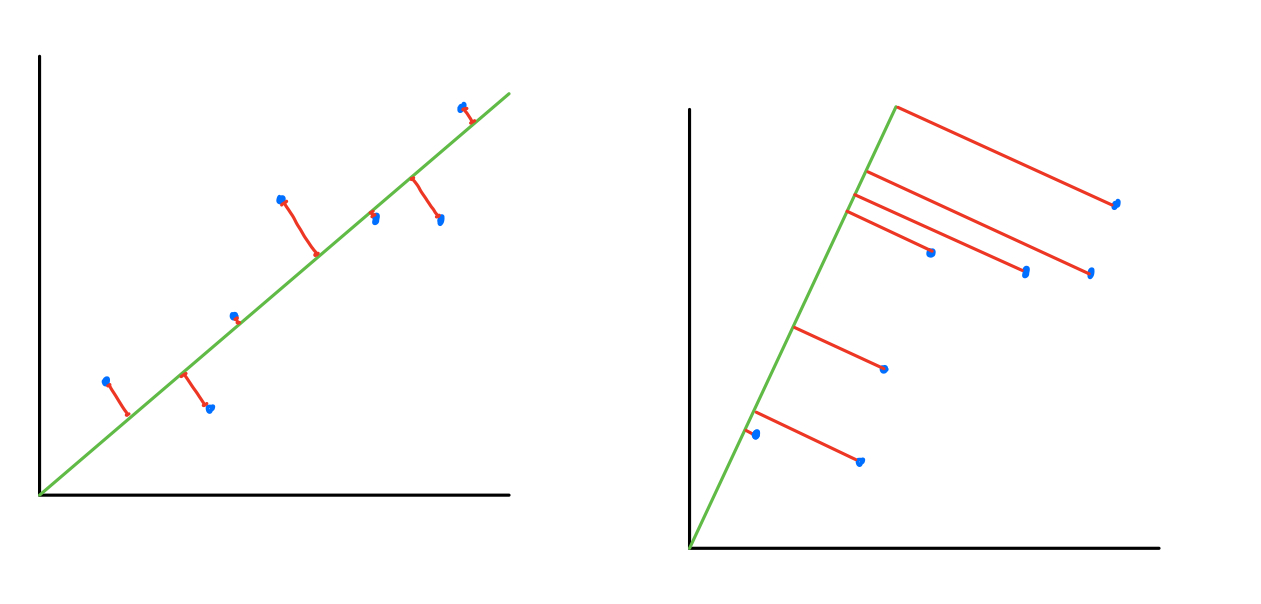
\includegraphics[scale=0.25]{images/minimum_error.jpg}
    \caption{Error Visualization}
\end{figure}

\vspace{2mm}
\noindent Suppose we rotate the original line from the first figure to the second, then we see that the error between each point and the line is much greater. Therefore the "best" principal component, the one which follows the data with most fidelity, is the one that minimizes the error. 

\vspace{2mm}
\noindent Formally, we want to minimize the mean squared error (sum of the error for each data point, divided by the total $N$ data points). We use the same notation as before: $\mathbf{x_n}$ is each data point, $N$ is the number of data points, and $\mathbf{\hat{x}}$ is the projection of $\mathbf{x}$ onto the subspace formed by the primary components. Then we seek to minimize the function: \
\begin{align*}
    \frac{1}{N}\sum_{n=1}^{N}||\mathbf{x_n - \hat{x}}||^2
\end{align*}

\subsubsection{Derivation}
\noindent Similar to the maximum variance formulation, suppose we have $N$ data points $\mathbf{x_n}$ in $\mathbb{R}^D$. Suppose further that we have an orthonormal basis for $\mathbb{R}^D$, defined $\{\mathbf{w_1, w_2, \cdots, w_D}\}$. Then we can express any data point as a linear combination of this basis:
\vspace{-5mm}
\begin{flalign*}
    \mathbf{x_n} &= c_1\mathbf{w_1} + \cdots + c_D\mathbf{w_D}\\
    &=\Sigma_{i = 1}^{D}c_{ni}\mathbf{w_i}
\end{flalign*}

\noindent Recall that the coordinates of $\mathbf{x_n}$ with respect to the basis $\{\mathbf{w_1, \cdots, w_D}\}$ is ($c, \cdots, c$).

\vspace{2mm}
\noindent\fbox{%
    \parbox{\textwidth}{%
        \textbf{Theorem.} The \textit{i}-th coordinate of vector $\mathbf{x}$ with respect to orthonormal basis $\{\mathbf{w_1, \cdots, w_D}\}$ is given by $\mathbf{x} \cdot \mathbf{w_i}$.

        \vspace{2mm}
        \begin{proof}
            This proof follows easily from the theorem giving the coordinates for an orthogonal basis: given orthogonal basis $\{\mathbf{u_1, \cdots, u_n}\}$, a coordinate $c_i$ is given by $\frac{x \cdot u_i}{u_i \cdot u_i}$.
        
            Then since the basis is made of vectors of unit length 1, and thus $u_i \cdot u_i = ||u_i||^2 = 1$, we have that coordinate $c_i = \mathbf{x \cdot w_i}$.
        \end{proof}
    }%
}

\vspace{2mm}
\noindent We therefore have that each coordinate $c_i = \mathbf{x_n \cdot w_i}$. Now suppose we define a center to the set of data points, which as we will see later, is typical when we standardize data. Let's define this as:

\vspace{-4mm}
\begin{align*}
    \mathbf{\bar{x}} = \frac{1}{N}\Sigma_{i = 1}^{N}\mathbf{x_i}
\end{align*}

\noindent Then we have:
\[
\begin{minipage}{.5\linewidth}
  \centering
  $
  \setstretch{1.5}
  \begin{array}{l@{{}\mathrel{=}{}}l}
    \mathbf{x_n} & c_1\mathbf{w_1} + \cdots + c_D\mathbf{w_D}\\[\jot]
    &\Sigma_{i = 1}^{D}c_{ni}\mathbf{w_i}\\[\jot]
    &\Sigma_{i=1}^{D}\mathbf{(x_n \cdot w_i)w_i}\\[\jot]
    &\mathbf{\bar{x}} + \Sigma_{i=1}^{D}(\mathbf{x_n \cdot w_i)w_i - \bar{x}}\\[\jot]
    &\mathbf{\bar{x}} + \Sigma_{i=1}^{D}(\mathbf{x_n \cdot w_i)w_i} - \Sigma_{i=1}^{D}(\mathbf{\bar{x} \cdot w_i)w_i}\\
  \end{array}$
\end{minipage}%
\begin{minipage}{.35\linewidth}
  \centering
  $
  \setstretch{1.5}
  \begin{array}{r}
    \\[\jot]
    \\[\jot]
    \text{Substituting in known value.}\\[\jot]
    \text{Add and subtract }\mathbf{\bar{x}}\\[\jot]
    \\
  \end{array}$
\end{minipage}
\]

\noindent Note $\mathbf{\bar{x}}$ is already in $\mathbb{R}^D$, so projection onto the basis of $\mathbb{R}^D$ will just be itself.

\vspace{2mm}
\noindent
\[
\begin{minipage}{.5\linewidth}
  \centering
  $
  \setstretch{1.5}
  \begin{array}{l@{{}\mathrel{=}{}}l}
    &\mathbf{\bar{x}} + \Sigma_{i=1}^{D}(\mathbf{x_n \cdot w_i - \bar{x} \cdot w_i)w_i}\\[\jot]
    &\mathbf{\bar{x}} + \Sigma_{i=1}^{D}((\mathbf{x - \bar{x}}) \cdot \mathbf{w_i})\mathbf{w_i}\\[\jot]
    &\mathbf{\bar{x}} + \Sigma_{i = 1}^{D}z_{i}\mathbf{w_i}
  \end{array}$
\end{minipage}%
\begin{minipage}{.35\linewidth}
  \centering
  $
  \setstretch{1.5}
  \begin{array}{r}
    \text{Combining summations.}\\[\jot]
    \\[\jot]
    \text{Let }z_{i} = (\mathbf{x - \bar{x}}) \cdot \mathbf{w_i}.
  \end{array}$
\end{minipage}
\]

\noindent Similarly, our projection of $\mathbf{x_n}$ onto a subspace of $k$ dimensions, instead of $D$, would simply be $\mathbf{\hat{x}} = \mathbf{\bar{x}} + \Sigma_{j=1}^{k}z_{j}\mathbf{w_j}$. Now we can rewrite our formula for the mean squared error, which we want to minimize.

\vspace{2mm}
$
\setstretch{1.5}
\begin{array}{l@{{}\mathrel{=}{}}l}
    \frac{1}{N}\sum_{n=1}^{N}||\mathbf{x_n - \hat{x}}||^2 & \frac{1}{N}\sum_{n=1}^{N}||\mathbf{x_n} - (\mathbf{\bar{x}} + \Sigma_{j=1}^{k}z_{j}\mathbf{w_j})||^2\\
    \text{We substitute in values that we know.} & \frac{1}{N}\sum_{n=1}^{N}||(\mathbf{\bar{x}} + \Sigma_{i = 1}^{D}z_{i}\mathbf{w_i}) - (\mathbf{\bar{x}} + \Sigma_{j=1}^{k}z_{j}\mathbf{w_j})||^2\\
    \text{Canceling terms.}&\frac{1}{N}\sum_{n=1}^{N}||\Sigma_{i = 1}^{D}z_{i}\mathbf{w_i}) - \Sigma_{j=1}^{k}z_{j}\mathbf{w_j}||^2\\
    \text{Simplifying the sum.}&\frac{1}{N}\sum_{n=1}^{N}||\Sigma_{i = k+1}^{D}z_{i}\mathbf{w_i}||^2\\
    \text{Dot product of self is length, squared.}&\frac{1}{N}\Sigma_{n=1}^{N}(\Sigma_{i=k+1}^{D}z_i\mathbf{w_i})\cdot(\Sigma_{i=k+1}^{D}z_i\mathbf{w_i})\\
\end{array}$

\vspace{2mm}
\noindent Now we note that a dot product of a sum of vectors can be calculated by summing the dot product of the vectors of the same "index", and then each pairing of the vectors that have different indices (which is represented with the double sum). This is because dot product is distributive.

$
\setstretch{1.5}
\begin{array}{l@{{}\mathrel{=}{}}l}
    &\frac{1}{N}\Sigma_{n=1}^{N}(\Sigma_{i=k+1}^{D}z_i\mathbf{w_i}\cdot\mathbf{w_i}z_i + \Sigma_{i=k+1}^{D} \Sigma_{j=k+1}^{D}(i\neq j)z_i\mathbf{w_i \cdot w_j}z_j)\\
    \text{Orthogonal $\rightarrow$ dot product is zero}&\frac{1}{N}\Sigma_{n=1}^{N}(\Sigma_{i=k+1}^{D}z_{i}^2)\\
    \text{Substitute value of $z$}&\frac{1}{N}\Sigma_{n=1}^{N}(\Sigma_{i=k+1}^{D}[(\mathbf{x_n - \bar{x}}) \cdot \mathbf{w_i}]^2)\\
    \text{Expand.}&\frac{1}{N}\Sigma_{n=1}^{N}(\Sigma_{i=k+1}^{D}[(\mathbf{x - \bar{x}})\cdot \mathbf{w_i}][(\mathbf{x - \bar{x}})\cdot \mathbf{w_i}])\\
    \text{Definition of dot product.}&\frac{1}{N}\Sigma_{n=1}^{N}(\Sigma_{i=k+1}^{D}\mathbf{w_{i}^{T}(x-\bar{x})(x-\bar{x})^{T}w_i})\\
    \text{Switch order of summation.}&\Sigma_{i=k+1}^{D}\mathbf{w_{i}^{T}}(\frac{1}{N}\Sigma_{n=1}^{N}\mathbf{(x_n - \bar{x})(x-\bar{x})^{T}})\mathbf{w_i}\\
    \text{Definition of covariance matrix.}&\Sigma_{i=k+1}^{D}\mathbf{w_{i}^{T}Sw_i}
\end{array}$

\hfill [Inspired by derivation from Sontag (7)]


\vspace{2mm}
\noindent We must now minimize this expression, which looks really familiar to the expression from the maximum variance formulation. We again apply the method of Lagrange multipliers, supposing that $D = 2, k = 1$ to simplify the method. Then our expression of mean squared error is: $f(\mathbf{w}) = \mathbf{w_{2}^{T}Sw_{2}}$.

\vspace{2mm}
\noindent Since our basis vectors are still unit vectors, we can again make our $g(\mathbf{w}) = 1 - \mathbf{w^{T}w} = 0$. Then we maximize $L(\mathbf{w}, \lambda) = \mathbf{w_{2}^{T}Sw_{2}} + \lambda(1-\mathbf{w_{2}^{T}w_2})$. Note this is the exact same equation as in the maximum variance formulation, so we will again get that $\mathbf{Sw = \lambda w}$.

\vspace{2mm}
\noindent This tells us two important things. First, we confirm that the choice of possible components to count as our primary ones are indeed eigenvectors of the covariance matrix. Secondly, we note that our mean squared error simplifies:

\begin{center}
    \setstretch{1.5}
    $\begin{array}{l@{{}\mathrel{=}{}}l}
        \Sigma_{i=k+1}^{D}\mathbf{w_{i}^{T}Sw_{i}} & \Sigma_{i=k+1}^{D}\lambda \mathbf{w_{i}^{T}w_{i}}\\
        &\Sigma_{i=k+1}^{D}\lambda
    \end{array}$
\end{center}

\vspace{2mm}
\noindent This is the sum of the eigenvalues corresponding to eigenvectors NOT chosen to be primary components. Therefore, mean squared error is minimized when we choose eigenvectors with the largest eigenvalues to be our primary components!
\subsection{Application}

Now that we've explored the reasoning and general application of PCA, we will give a brief overview of its application to data sets.

\begin{enumerate}
    \item \textbf{Standardize.} Before PCA, we want to standardize the range of the variables so that each contributes equally. Prior to standardization, variables with large ranges will always dominate over those with smaller ranges, even if they should contribute equally to how we measure a data point. For instance, the scale of population size to an individual's age differ by an order of magnitude, even if they may contribute equally to, say, the average health of a city. Thus, for each value of the variables, we subtract the mean and divide by the standard deviation to standardize the data. 

    \item \textbf{Compute Covariance Matrix.} As defined earlier, the covariance matrix allows us to see the relationship between the variables.

    \item \textbf{Compute Eigenvectors and Eigenvalues.} As detailed in the Maximum Variance Formulation proof, we calculate the eigenvectors and eigenvalues of the covariance matrix. The eigenvectors are the principal components, and the eigenvalue of a principal component denotes how much of the variance the component captures. Therefore, the components with the smallest eigenvalues are the least relevant.
\end{enumerate}

\noindent PCA can be applied in many contexts where there's a large amount of data, not all necessary, such that it can be heavily simplified and reduced before analysis.

\subsection{Example in Python}

\noindent We now provide a simple example of PCA in data science. Broadly, we are given a set of many images, each of which is an article of clothing. Each of these images is 784 pixels, which is represented as a row vector of length 784. From there, we can standardize the data: in this case, we standardize the set of pixels to have mean 0 and standard deviation 1. We then compute the principal components (with a single function call) and project the data points onto the components, which we represent with a scatter plot.

\vspace{1mm}
\noindent We include the code here, including explanations below each code block.


\begin{lstlisting}
import pandas as pd
from sklearn.preprocessing import StandardScaler
from sklearn.decomposition import PCA
import matplotlib.pyplot as plt
import seaborn as sns

# load dataset into Pandas DataFrame
df = pd.read_csv("fashion-mnist_train.csv")
\end{lstlisting}

\noindent We load the relevant libraries. Then we read in the Fashion-MNIST data set. The MNIST set is commonly used to test and train machine learning algorithms, making this example very applicable in the real world. The data set is in the form of a comma-separated value (CSV) file, which we convert into a dataframe (df), which is basically a table, using the pandas library. When we print out the first 6 lines of this dataframe (print(df.head())), the data looks like this: 

\vspace{2mm}
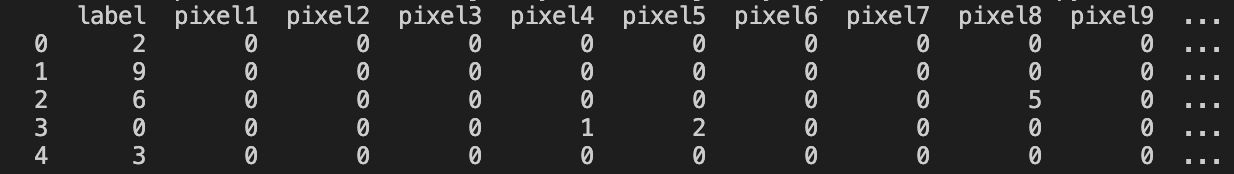
\includegraphics[scale=0.5]{images/df_head.png}

\vspace{2mm}
\noindent Note that the 'label' column is all numbers, which actually correspond to the types of articles of clothing in the image (displayed as the pixels in that row). We will later transcribe the type of clothing from these integer in the legend.

\begin{lstlisting}
# Separating out the features
x = df.drop('label', axis=1).values
# Standardizing the features
x = StandardScaler().fit_transform(x)
\end{lstlisting}

\noindent Here, we first drop the column named 'label' and grab the values without the column names ('pixel1', 'pixel2', etc). We then standardize the data, as explained above, by simply calling fit\_transform().

\begin{lstlisting}
# Perform PCA
pca = PCA(n_components=2)
principalComponents = pca.fit_transform(x)
principalDf = pd.DataFrame(data = principalComponents, columns = ['principal component 1', 'principal component 2'])
\end{lstlisting}

\noindent We prepare the PCA model to calculate for 2 primary components. Then, we fit this model to our data from above (x) and run PCA on it. This will result in the data being projected onto the principal components. Finally, we put this data back in a dataframe.

\begin{lstlisting}
# Label the legend appropriately
labels = {0: 'T-shirt/top', 1: 'Trouser', 2: 'Pullover', 3: 'Dress', 4: 'Coat', 5: 'Sandal', 6: 'Shirt', 7: 'Sneaker', 8: 'Bag', 9: 'Ankle boot'}
df['label'] = [labels[lbl] for lbl in df['label']]
finalDf = pd.concat([principalDf, df[['label']]], axis = 1)
\end{lstlisting}

\noindent We provide a dictionary mapping the integer representation of each type of clothing to the readable string version of that article of clothing. We then replace the entire 'label' column of the original dataframe (where the data was initially loaded) with the string versions, instead of the integers. Finally, we create our final dataframe by concatenating the data from the PCA with our revised labels. (Recall that we originally dropped the 'label' column before we ran PCA on the data set.)

\begin{lstlisting}
fig, ax = plt.subplots(1)
fig.set_size_inches(8,8)
ax.set_xlabel('Principal Component 1', fontsize = 15)
ax.set_ylabel('Principal Component 2', fontsize = 15)
ax.set_title('2 component PCA', fontsize = 20)
sns.scatterplot(data=finalDf, x='principal component 1', y='principal component 2', hue='label', ax=ax, alpha=0.5, palette="tab10")
ax.grid()
plt.show()
\end{lstlisting}

\noindent We plot the data as a scatter plot. Since this isn't particularly applicable to PCA, we will not discuss this code line-by-line.

\noindent The resulting plot after PCA appears as below:

\begin{figure}[h]
    \centering
    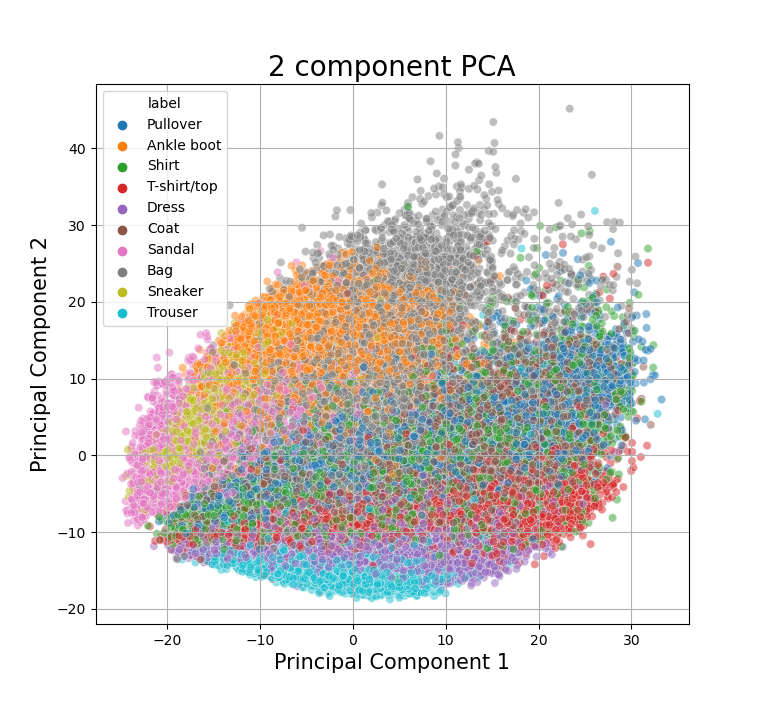
\includegraphics[scale=0.65]{images/fashionMNIST_plot.png}
    \caption{PCA on MNIST Fashion Data}
\end{figure}

\noindent We can see that after projection onto these principle components, the same articles of clothing appear grouped together. With more principal components, we might be able to further the separation and create more distinct groups for each type of clothing.

\begin{lstlisting}
print(pca.explained_variance_ratio_)
\end{lstlisting}

\noindent As it stands, these two primary components account for about 35\% of the data variance. The array displays corresponding variances to each component:

\begin{center}
  
\includegraphics{images/variance.png}  
\end{center}

\noindent With this example in mind, we can continue to extend the application of PCA to facial recognition.

\pagebreak

\section{Facial Recognition Algorithms}
Going back to our question we proposed in the introduction, how do we distinguish faces? Facial recognition has been a problem that has fascinated scientists and philosophers for centuries. Though we do not realize it, we perform amazing feats on a daily basis; we can recognize thousands of faces at a glance and even with changes in lighting, expression, aging or accessories like glasses. This ease does not translate to computational models, and many have tried to create detection algorithms.


\subsection{Prior Research}
Early work in facial recognition used the strategy of detecting individual facial features (ex. eyes, nose, mouth) and creating a model based on the position, size, and relationship among those features. This strategy is difficult to extend to different views of the face and is quite fragile (Carey \& Diamond, 1977).
Variations of this strategy have been used in the past. Woodrow Bledsoe was the first to attempt facial recognition with a hybrid system. The parameters used to classify faces were normalized distances and ratios among distinct points on the face (ex. eye corners, mouth corners, chin point) (Bledsoe, 1966). Others have used a set of geometric parameters and performed pattern recognition. 

\subsection{Eigenfaces}
Turk and Pentland (1991) detail a different approach in their paper, \textit{Eigenfaces for Recognition}. Their general approach was to extract the most important and relevant information in a face image, allowing all faces to be encoded with the most important aspects of a face and compared. Following PCA, we want to find the principal components of the distribution of faces or specifically, the eigenvectors corresponding to the covariance matrix of a set of training images. These eigenvectors describe the variance in the set of images. The authors specifically define a term \textit{eigenfaces}:


\vspace{3mm}

\noindent\fbox{%
    \parbox{\textwidth}{%
        \textbf{Definition.} \textit{Eigenface}. The image display of an eigenvector calculated from the covariance matrix of the set of images. See Figure 3 for examples of eigenfaces. 
    }%
}
\begin{figure}[h]
    \centering
    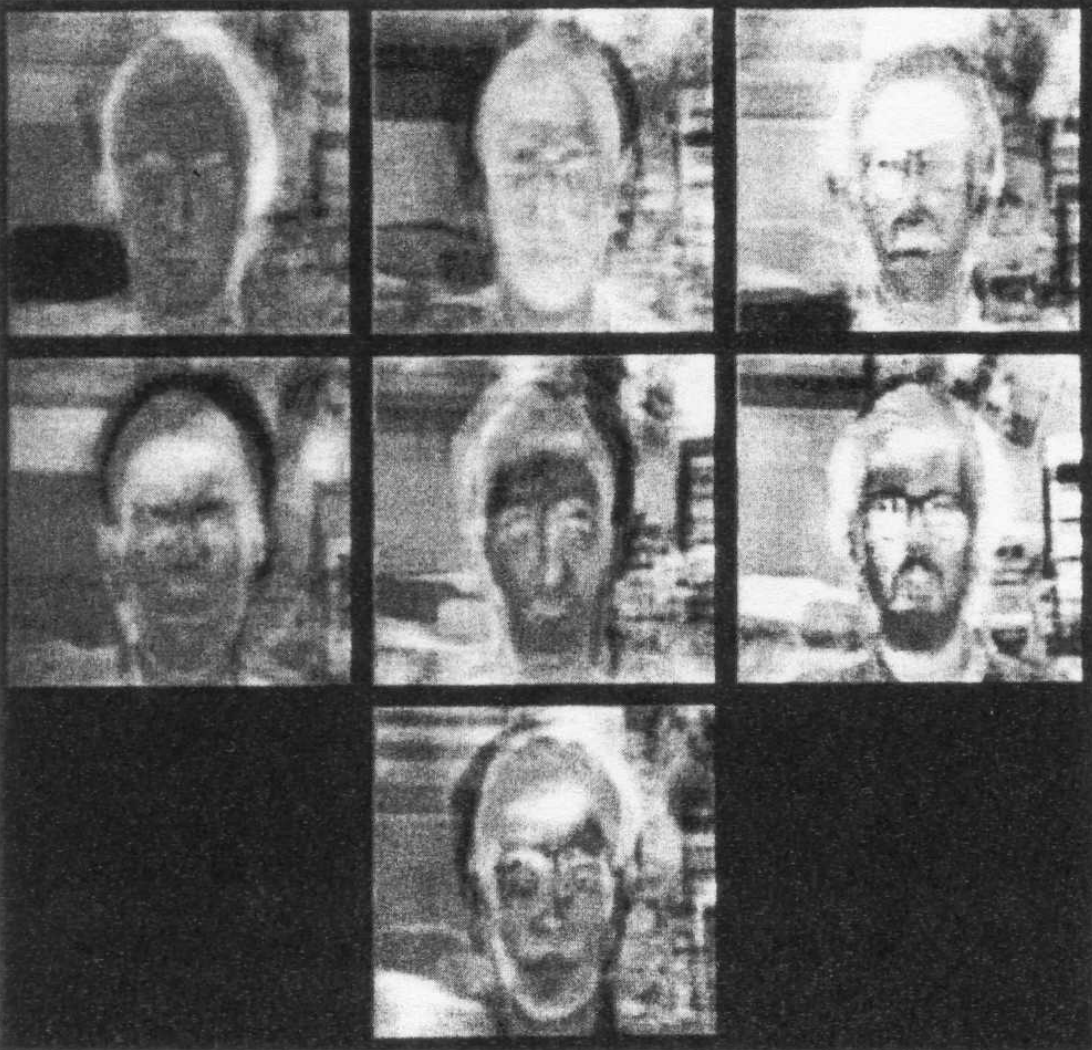
\includegraphics[scale=0.18]{images/eigenface.png}
    \caption{Eigenface Examples from Turk \& Pentland, 1991}
\end{figure}

\noindent Because eigenfaces span the subspace of face images, this means every face can be expressed as a linear combination of the eigenfaces. Moreover, every image can be approximated to a very close degree by using only the eigenfaces with the highest eigenvalues (which we proved earlier captures the most variance). This leads us to define the space of face images as a \textit{facespace}.

\vspace{3mm}

\noindent\fbox{%
    \parbox{\textwidth}{%
        \textbf{Definition.} \textit{Facespace}. The $M$-dimensional subspace of all possible face images, spanned by the $M$ best eigenfaces. 
    }%
}

\vspace{3mm}

\noindent With the general approach explained, let us detail the process mathematically. 

\subsubsection{Obtain Initial Face Images}

First, get a training set of $M$ face images of the known individuals including several for each person with variation in lighting and expression. Each image can be expressed as an $N \times N$ array of 8-bit intensity values. That is, we have $N^2$ values between 0 and 256 representing each pixel of the image. We can also express each image as a vector with a length of $N^2$.

\subsubsection{Calculate Eigenfaces}
Let the training set of images be $N^2$ vectors $I_1,I_2,I_3,...,I_M$. Following the procedure of PCA, we want to first standardize the range of our variables. We can calculate the "average face" that is, the mean of the face image vectors:

$$I_\mu = \frac{I_1 + I_2 + I_3 +...+ I_M}{M}$$

\noindent Now, we define our standardized vectors as $\Phi_1, \Phi_2, \Phi_3,...,\Phi_M$, where
$$\Phi_j = I_j - I_\mu$$

\noindent Following our definition of a Variance-Covariance Matrix, we can define the covariance matrix of the face set to be
$$S = \frac{1}{M}\sum_{j=1}^{M}\Phi_j\Phi_j^T$$
\noindent Because we have standardized our data, the mean of our vectors $\Phi_1, \Phi_2, \Phi_3,...,\Phi_M$ is 0. Therefore, defining $A = [\Phi_1 \Phi_2 \Phi_3 ... \Phi_M]$, we can express $S$ as
$$S = AA^T$$

\noindent We would like to find the eigenvectors, $u_k$ and eigenvalues $\lambda_k$ associated with this matrix. Because our covariance matrix, $S$, is an $N^2 \times N^2$ matrix, this is incredibly large and hard to deal with when working with typical image sizes. Thus, we want to use a simpler way to calculate the eigenvectors. Note that if the number of images we have, $M$, is less than the dimension of the image space $N^2$, many of the eigenvectors will have the associated eigenvalue of 0 which does not give us any information. Thus, $S$ will only have $M-1$ meaningful eigenvectors. This means that we can calculate the eigenvectors for an $M \times M$ matrix, then take linear combinations of the face images to get the eigenvectors of $S$. Consider the eigenvectors of matrix $A^TA$. By definition of eigenvectors, let $v_i$ be an eigenvector of eigenvalue $\lambda_i$ such that 
$$A^TAv_i = \lambda_iv_i$$
\noindent If we multiply each side by $A$ we get 
$$AA^TAv_i = \lambda_iAv_i$$
\noindent This means that by definition of eigenvectors, $Av_i$ is an eigenvector for matrix $AA^T$ (our covariance matrix $S$) with eigenvalue $\lambda_i$. Let $B = A^TA$ and find the $M$ eigenvectors and eigenvalues of $B$, $v_1,...,v_M$. These eigenvectors represent the weights of vectors $\Phi_1, \Phi_2,..., \Phi_M$, so we can create the eigenfaces $u_1,...,u_M$ as follows:
$$u_i = \sum_{k=1}^{M}v_{ik}\Phi_k$$

\noindent We now have eigenfaces $u_1,...,u_M$ with associated eigenvalues $\lambda_1,...,\lambda_M$ that will allow us the rank eigenfaces by how much variation they capture.

\subsubsection{Use Eigenfaces for Recognition}
Having developed a way to computationally describe faces, facial recognition becomes a problem of pattern recognition. Given our set of training images, we have a certain number of "known individuals" that we can call face classes. Each face class, $\Omega_i$, is calculated by averaging the eigenface representations of images of the same person. Say we are given a new face image $F$ and we want to match the face to a known face. We must first find the eigenface weights for $F$. Standardize $F$ to get $\Phi_F = F - I_\mu$. Now, we can calculate the weights $\omega_1, \omega_2, ..., \omega_M$ like so:
$$\omega_k = u_k^T\Phi_F$$

\noindent We can write these weights as a vector $\Omega^T = [\omega_1, \omega_2, ..., \omega_M]$. Now we can compare $\Omega$ with $\Omega_i$ for each face class. To account for some error, we can set some error threshold $\theta_\epsilon$, then find the face class that minimizes the euclidean distance between the two vectors, $\epsilon_k$, that is below the threshold $\theta_\epsilon$. $\epsilon_k$ is calculated like so
$$\epsilon_k^2 = ||(\Omega - \Omega_k)||^2$$

\noindent If no $\epsilon_k$ is under the threshold, we can say this image $F$ is a new unknown face and perhaps create a new face class with it. However to distinguish unknown faces from images that look nothing like a face, we can measure distance to the face space. The distance $\epsilon$ between the image and the face space can be calculated using the standardized image, $\Phi_F$, and its projection on the face space, $\Phi_\mu = \omega_1u_1 + ... + \omega_Mu_M$. 

$$\epsilon^2 = ||(\Phi_F - \Phi_\mu)||^2$$


\noindent There are typically 4 outcomes of this pattern matching algorithm: 
\begin{itemize}
    \item \textbf{Near face space ($\epsilon < \theta_\epsilon$) and near face class ($\epsilon_k < \theta_\epsilon$)}: This means our image matches a known face, $k$.
    \item \textbf{Near face space ($\epsilon < \theta_\epsilon$) and distant from face class ($\epsilon_k \geq \theta_\epsilon$)}: This means we have an unknown face. 
    \item \textbf{Distant from face space ($\epsilon \geq \theta_\epsilon$) and near face class ($\epsilon_k < \theta_\epsilon$)}: This means we don't have a face, but the pattern is close to a face class. This is usually a false positive. 
    \item \textbf{Distant from face space ($\epsilon \geq \theta_\epsilon$) and distant from face class ($\epsilon_k \geq \theta_\epsilon$)}: This means we don't have a face and the pattern didn't match a face class either.
\end{itemize}

\noindent Based on the euclidean distance of some image to the face space (the subspace of face images), we can detect if the image is a face. Based on euclidian distance of the image to a specific face class, we can detect if it is a known individual in our training set. 

\subsubsection{Takeaway}
Here is a brief summary of the steps to perform facial recognition using eigenfaces:
\begin{enumerate}
    \item Get a training set of face images.
    \item Standardize and calculate its covariance matrix, $S$.
    \item Find the meaningful eigenvectors and eigenvalues of the $B$ matrix.
    \item Apply the eigenvectors to the face images to produce eigenfaces.
    \item Calculate face classes for each known individual and choose an error threshold $\theta_\epsilon$.
    \item For a new input image, calculate its eigenface weights and compare its distance with the face classes and its distance from the facespace. If $\epsilon < \theta_\epsilon$ and $\epsilon_k < \theta_\epsilon$, we have a match with face $k$. If $\epsilon < \theta_\epsilon$ and there is no close face class, we have an unknown face. 
\end{enumerate}

This method is limited by many assumptions that may not be valid in a real application. For one, we assume these face images are centered. However, this method can be extended to use the facespace to locate the face in an image. There are many other issues that may cause problems with a functional implementation of this algorithm such as head orientation, head size, image background, etc. that many are working to address. Still, this research provides a robust base to solve the problem of facial recognition. 

\section{Conclusion}
We have now walked through the basics of Principal Component Analysis: from its derivation to its applications at both basic and higher levels. Evidently, PCA is a powerful tool that allows us to model data with less noise through dimension reduction. We see that it's very effective at helping us find patterns from complex multidimensional data, not only from the main "axes" of data, but also physically in how we can use the principal components to graph data. As such, PCA serves as a foundational block of modern machine learning, and its applications are only beginning to be tapped as interest in artificial intelligence/machine learning continues to grow.

\pagebreak
\begin{thebibliography}{10}

\bibitem{Bledsoe} Bledsoe, W. W. (1966). \emph{The model method in facial recognition}. Panoramic Research Inc. 
\bibitem{Blitzstein} Blitzstein J. K. \& Hwang J. (2019). \emph{Introduction to probability}. CRC Press/Taylor \& Francis Group.
\bibitem{Carey} Carey \& Diamond R. (1977). \emph{From Piecemeal to Configurational Representation of Faces}. Science (American Association for the Advancement of Science). 
\bibitem{Lay} Lay D. C. Lay S. R. \& McDonald J. (2016). \emph{Linear algebra and its applications (Fifth)}. Pearson. 
\bibitem{Peck} Peck R. Olsen C. \& Devore J. L. (2008). \emph{Introduction to statistics and data analysis (3rd ed.)}. Thomson Brooks/Cole.
\bibitem{Sankar} Sankar, A. (2021, September 29). \emph{Principal Component Analysis Part 1: The different formulations.} Medium.
\bibitem{Sontag} Sontag, D. (n.d.). \emph{Dimensionality Reduction, Lecture 25}. New York University. 
\bibitem{Stewart} Stewart J. (2012). \emph{Multivariable calculus (7th ed.)}. Brooks/Cole.
\bibitem{Trench} Trench, W. (2012, November). The method of Lagrange multipliers.
\bibitem{Turk} Turk, M., \& Pentland, A. (1991). \emph{Eigenfaces for Recognition}. Journal of Cognitive Neuroscience.

\end{thebibliography}

\end{document}
